%%%%%%%% ICML 2026 POSITION PAPER %%%%%%%%%%%%%%%%%

\documentclass{article}

% Recommended packages
\usepackage{microtype}
\usepackage{graphicx}
\usepackage{subcaption}
\usepackage{booktabs}
\usepackage{hyperref}
\usepackage{multirow}
\usepackage{xcolor}
\usepackage{float}
\usepackage[section]{placeins}
\usepackage{tikz}
\usetikzlibrary{shapes.geometric, arrows, positioning, fit, backgrounds, patterns}
\usepackage{pgfplots}
\pgfplotsset{compat=1.18}

\newcommand{\theHalgorithm}{\arabic{algorithm}}

% Use the following line for the initial blind version submitted for review:
\usepackage{icml2026}

\usepackage{amsmath}
\usepackage{amssymb}
\usepackage{mathtools}
\usepackage{amsthm}

\usepackage[capitalize,noabbrev]{cleveref}

%%%%%%%%%%%%%%%%%%%%%%%%%%%%%%%%
% THEOREMS
%%%%%%%%%%%%%%%%%%%%%%%%%%%%%%%%
\theoremstyle{plain}
\newtheorem{theorem}{Theorem}[section]
\newtheorem{proposition}[theorem]{Proposition}
\theoremstyle{definition}
\newtheorem{definition}[theorem]{Definition}

\icmltitlerunning{Position: Beyond Benchmark Gaming}

\begin{document}

\twocolumn[
  \icmltitle{Position: Beyond Benchmark Gaming - A Call for Dynamic Out-of-Distribution Evaluation of Language Models}

  \begin{icmlauthorlist}
    \icmlauthor{Anonymous Author(s)}{anon}
  \end{icmlauthorlist}

  \icmlaffiliation{anon}{Anonymous Institution}

  \icmlcorrespondingauthor{Anonymous Author(s)}{anonymous@example.com}

  \icmlkeywords{Language Models, Benchmarks, Test-Time Learning, Out-of-Distribution Generalization, Esoteric Programming Languages}

  \vskip 0.3in
]

\printAffiliationsAndNotice{}

\begin{abstract}
This position paper argues that \textbf{current static LLM benchmarks incentivize optimization toward specific test distributions rather than genuine generalization, and that the machine learning community should adopt dynamic out-of-distribution benchmarks that evaluate test-time learning capabilities}. We present empirical evidence showing benchmark contamination significantly inflates reported performance, and demonstrate through experiments on esoteric programming languages that state-of-the-art models achieve less than 14\% accuracy on truly out-of-distribution tasks despite near-perfect performance on mainstream benchmarks. Critically, few-shot learning provides no significant benefit for OOD tasks, while agentic systems achieve 2--3$\times$ improvement through efficient context management and interpreter feedback. We argue that the rigid train-test separation paradoxically prevents evaluation of the very capabilities that define intelligence. \textbf{Our position advocates for benchmarks using esoteric programming languages that are economically irrational to include in training data, combined with test-time learning protocols that measure learning efficiency and feedback utilization.} The resulting EsoLang benchmark measures genuine transferable reasoning skills---mimicking how humans acquire new abilities by applying general knowledge to unfamiliar domains---rather than rewarding memorization of training data.
\end{abstract}

\section{Introduction}

The rapid advancement of Large Language Models (LLMs) has been marked by increasingly impressive benchmark scores: 95\%+ on GSM8k \cite{cobbe2021training}, near-human performance on MMLU \cite{hendrycks2021measuring}, and state-of-the-art results on HumanEval \cite{chen2021evaluating}. Yet beneath these headline numbers lurks a troubling reality: models are being optimized for benchmarks rather than capabilities, and the machine learning community's evaluation paradigm may be fundamentally misaligned with the goal of developing genuinely intelligent systems.

\textbf{Our position is that static benchmarks have reached diminishing returns as evaluation tools for language model capabilities, and that the community should adopt dynamic out-of-distribution benchmarks using domains like esoteric programming languages, combined with test-time learning protocols that measure the ability to acquire new skills during inference rather than retrieve memorized patterns.}

Recent empirical work reveals the extent of benchmark contamination and design flaws. Zhang et al.~\cite{zhang2024careful} demonstrated that models show systematic overperformance on GSM8k compared to the contamination-free GSM1k benchmark, with accuracy drops of up to 8\% observed across model families, providing evidence of systematic overfitting. Sainz et al.~\cite{sainz2023nlp} found widespread contamination across NLP benchmarks, while Deng et al.~\cite{deng2024investigating} documented significant memorization affecting benchmark scores across model families.

Beyond contamination, recent analysis reveals fundamental design flaws in prominent benchmarks. Chandak et al.~\cite{chandak2025answer} demonstrate that multiple-choice questions from popular benchmarks can often be answered without even seeing the question. In MMLU-Pro's chemistry and physics subsets, simply selecting answers with certain formatting patterns (e.g., leading spaces) yields surprisingly high accuracy. More strikingly, fine-tuning an 8B parameter model on answer distributions alone, without any access to questions, achieves 41\% accuracy on MMLU-Pro. For MMMU-Pro, a multimodal benchmark, models achieve 51\% accuracy without the question \textit{and} without the image. These findings suggest that reported progress may substantially overstate actual capability improvements, as models exploit statistical shortcuts rather than demonstrating genuine understanding.

The benchmark gaming crisis stems from three interrelated factors. First, economic pressure creates enormous incentives for achieving state-of-the-art scores, with billion-dollar valuations tied to benchmark leaderboard positions. Second, data contamination occurs inevitably as benchmarks become public and appear in training corpora through web scraping or deliberate inclusion \cite{zhou2023dont, xu2024benchmarking}. Third, the community's response of creating ``retro-holdout'' variants like GSM1k represents a reactive rather than preventive approach that fails to address the fundamental problem: static benchmarks are gameable by design. This creates a self-perpetuating cycle illustrated in Figure~\ref{fig:cycle}.

\begin{figure}[t]
\begin{center}
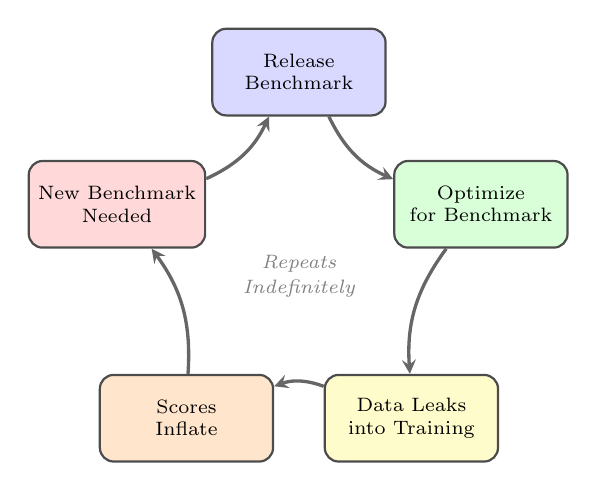
\begin{tikzpicture}[
    scale=0.9,
    node distance=1.4cm,
    stage/.style={rectangle, rounded corners=5pt, draw=black!70, line width=0.8pt, minimum width=2.2cm, minimum height=1.1cm, font=\scriptsize, align=center},
    arrow/.style={->, >=stealth, line width=1.2pt}
]
% Nodes in a pentagon
\node[stage, fill=blue!15] (n1) at (90:2.7cm) {Release\\Benchmark};
\node[stage, fill=green!15] (n2) at (18:2.7cm) {Optimize\\for Benchmark};
\node[stage, fill=yellow!20] (n3) at (-54:2.7cm) {Data Leaks\\into Training};
\node[stage, fill=orange!20] (n4) at (-126:2.7cm) {Scores\\Inflate};
\node[stage, fill=red!15] (n5) at (162:2.7cm) {New Benchmark\\Needed};

% Arrows with consistent style
\draw[arrow, black!60] (n1) to[bend right=20] (n2);
\draw[arrow, black!60] (n2) to[bend right=20] (n3);
\draw[arrow, black!60] (n3) to[bend right=20] (n4);
\draw[arrow, black!60] (n4) to[bend right=20] (n5);
\draw[arrow, black!60] (n5) to[bend right=20] (n1);

% Center annotation
\node[font=\scriptsize\itshape, gray] at (0,0) {Repeats};
\node[font=\scriptsize\itshape, gray] at (0,-0.35) {Indefinitely};
\end{tikzpicture}
\end{center}
\caption{The benchmark gaming cycle. This cycle has repeated with GLUE, SuperGLUE, MMLU, and continues today.}
\label{fig:cycle}
\end{figure}

Beyond contamination, we argue that the machine learning community's rigid adherence to strict train-test separation, while essential for traditional supervised learning, has become a constraint that prevents evaluation of the capabilities that truly matter for general intelligence. Consider how humans learn: a programmer learning Python who already knows Java does not memorize Python syntax beforehand. Instead, they learn through interaction with interpreters, documentation, and trial-and-error. A person solving a novel problem reasons from first principles and updates their understanding based on feedback. Humans learn continuously throughout their lives, acquiring new skills as needed.

Current benchmarks forbid exactly these learning mechanisms during evaluation. Models are expected to solve out-of-distribution problems without access to execution feedback, ability to update parameters or context based on test-time signals, or opportunity to learn from mistakes within a problem-solving session. This creates a fundamental mismatch: we evaluate models on their ability to retrieve memorized patterns rather than their ability to learn and reason, which are the very capabilities that define human intelligence.

\section{Related Work}

\textbf{Benchmark Contamination and Evaluation Integrity.} The problem of benchmark data appearing in training corpora has been extensively documented. Jacovi et al.~\cite{jacovi2023stop} proposed practical strategies for mitigating contamination, while Oren et al.~\cite{oren2024proving} developed methods for proving contamination in black-box models. Zhou et al.~\cite{zhou2023dont} and Xu et al.~\cite{xu2024benchmarking} quantified leakage across benchmark families. Bowman and Dahl~\cite{bowman2021fix} argued for fundamental reforms to NLU benchmarking, while Raji et al.~\cite{raji2021ai} critiqued the proliferation of narrow benchmarks. Ribeiro et al.~\cite{ribeiro2020beyond} introduced behavioral testing beyond accuracy metrics. Our work builds on these findings to argue that contamination is not merely a technical problem but a symptom of misaligned evaluation incentives.

\textbf{Code Generation and Program Synthesis.} HumanEval \cite{chen2021evaluating}, MBPP \cite{austin2021program}, and SWE-bench \cite{jimenez2024swebench} have driven progress in code generation. MultiPL-E \cite{cassano2023multipl} extended evaluation to multiple languages, DS-1000 \cite{lai2023ds1000} focused on data science, and AlphaCode \cite{li2022competition} tackled competitive programming. Code LLMs including CodeGen \cite{nijkamp2023codegen}, StarCoder \cite{lozhkov2024starcoder}, InCoder \cite{fried2023incoder}, CodeT5+ \cite{wang2023codet5}, and Code Llama \cite{roziere2024code} have achieved impressive results on these benchmarks. Program synthesis research \cite{gulwani2017program, ellis2021dreamcoder} provides theoretical foundations. However, all these benchmarks evaluate mainstream languages with abundant training data. Our proposal complements this work by introducing evaluation domains where memorization is impossible.

\begin{figure}[t]
\begin{center}
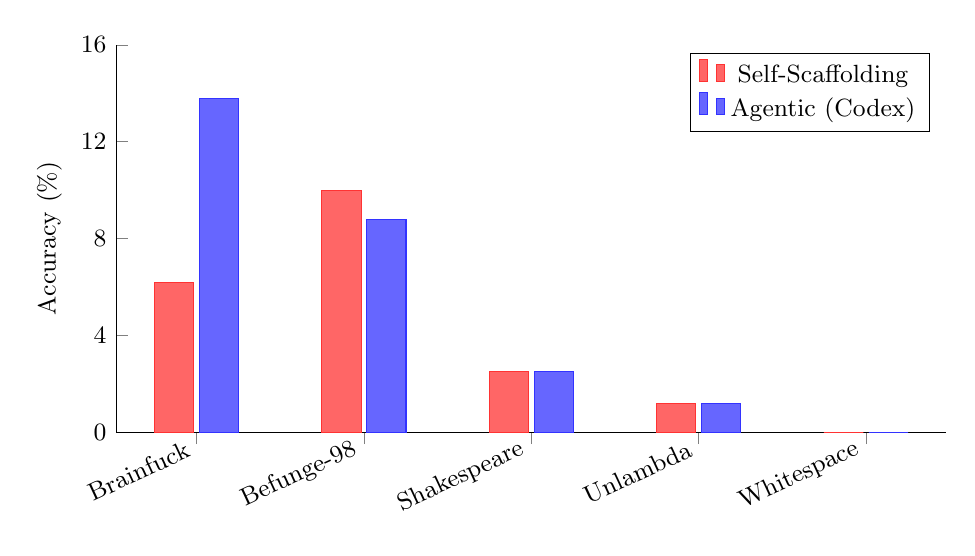
\begin{tikzpicture}[scale=1.0]
\begin{axis}[
    ybar,
    width=\columnwidth,
    height=6.5cm,
    ylabel={Accuracy (\%)},
    ylabel style={font=\small},
    symbolic x coords={Brainfuck, Befunge-98, Shakespeare, Unlambda, Whitespace},
    xtick=data,
    x tick label style={rotate=25, anchor=east, font=\small},
    ymin=0, ymax=16,
    ytick={0,4,8,12,16},
    yticklabel style={font=\small},
    bar width=0.5cm,
    legend style={at={(0.98,0.98)}, anchor=north east, font=\small},
    axis lines*=left,
    enlarge x limits=0.12,
]
\addplot[fill=red!60, draw=red!80] coordinates {
    (Brainfuck, 6.2) (Befunge-98, 10.0) (Shakespeare, 2.5) (Unlambda, 1.2) (Whitespace, 0)
};
\addplot[fill=blue!60, draw=blue!80] coordinates {
    (Brainfuck, 13.8) (Befunge-98, 8.8) (Shakespeare, 2.5) (Unlambda, 1.2) (Whitespace, 0)
};
\legend{Self-Scaffolding, Agentic (Codex)}
\end{axis}
\end{tikzpicture}
\end{center}
\caption{Best performance on esoteric languages. Agentic systems with IDE integration (Codex) achieve 13.8\% on Brainfuck---2$\times$ better than non-agentic approaches. For comparison, models achieve 85--92\% on equivalent problems in Python/Java.}
\label{fig:oodwall}
\end{figure}

\textbf{Out-of-Distribution Generalization and Domain Adaptation.} OOD generalization in NLP has been studied through CrossFit \cite{ye2021crossfit} and adversarial evaluation \cite{yang2023robustness}. Domain adaptation theory \cite{ben2010theory, ganin2016domain} and surveys \cite{wang2022generalizing} establish formal frameworks for understanding distribution shift. The transformer expressivity literature \cite{merrill2024expressive, anil2022exploring} and studies of compositional generalization \cite{dziri2024faith} provide theoretical grounding for understanding model limitations. Chollet's work on measuring intelligence \cite{chollet2019measure} and Mitchell's analysis of abstraction \cite{mitchell2021abstraction} inform our perspective on what evaluation should measure. Our empirical results on esoteric languages provide concrete evidence of OOD failure modes in state-of-the-art systems.

\textbf{Test-Time Adaptation and Continual Learning.} Test-time training \cite{sun2020test, liu2021ttt, gandelsman2022test} and adaptation \cite{wang2021tent} enable models to improve during inference. TTRL \cite{zuo2025ttrl} applies reinforcement learning at test time. CodeRL \cite{le2022coderl} uses RL for code generation. Recent work on efficient test-time reasoning~\cite{sharma2025think, sharma2025sequential} demonstrates that entropy-based early stopping and sequential reasoning can achieve 25--50\% computational savings while maintaining accuracy. Continual learning research \cite{kirkpatrick2017overcoming, scialom2022fine, wu2024continual} addresses catastrophic forgetting when learning new tasks. Scaling laws \cite{kaplan2020scaling, hoffmann2022training} inform understanding of model capacity. Our benchmark proposal provides a concrete testbed for evaluating these emerging test-time learning capabilities.

\section{The Case for Esoteric Programming Languages}

We propose esoteric programming languages (esolangs) as a principled solution to the benchmark gaming problem. Table~\ref{tab:paradigm} contrasts our dynamic OOD approach with static benchmarks across key dimensions.

\subsection{Economic Disincentive for Gaming}

It is economically irrational to pre-train or post-train on esoteric languages. These languages have minimal real-world utility---no deployment value justifies the training cost. Data collection costs are high relative to scarcity, and training on esolangs would harm performance on valuable mainstream tasks. Unlike traditional benchmarks where gaming provides competitive advantage, esolang benchmarks offer no return on investment for deliberate optimization.

\begin{table}[t]
\caption{Comparison of static vs.\ dynamic OOD benchmark paradigms.}
\label{tab:paradigm}
\vskip 0.05in
\begin{center}
\resizebox{\columnwidth}{!}{%
\begin{small}
\begin{tabular}{lcc}
\toprule
Aspect & Static Benchmarks & Dynamic OOD (Ours) \\
\midrule
Contamination Risk & High & Minimal \\
Gaming Incentive & High & None \\
Primary Measure & Retrieval & Reasoning \\
Test-Time Learning & Forbidden & Measured \\
Error Interpretability & Limited & High \\
Human Alignment & Weak & Strong \\
\bottomrule
\end{tabular}
\end{small}
}%
\end{center}
\end{table}

\subsection{Pure Reasoning Requirement}

Success on esoteric language tasks requires genuine reasoning: understanding computational primitives (loops, conditionals, state), mapping novel syntax to known semantics, leveraging documentation at inference time, and algorithmic reasoning rather than pattern matching. When a model succeeds on an esolang task, we can be confident it has engaged in actual reasoning rather than memorization.

\section{The EsoLang Benchmark: A Concrete Proposal}

To ground our position in concrete evaluation, we have developed the \textbf{EsoLang Benchmark Dataset}, a comprehensive suite of 80 programming problems spanning four difficulty levels, designed specifically for evaluating OOD generalization on esoteric programming languages. This benchmark serves as a proof-of-concept for our proposed evaluation paradigm and is being released to encourage community adoption.

\subsection{Dataset Structure and Design}

The benchmark consists of 80 problems distributed across four difficulty tiers: 20 easy, 20 medium, 20 hard, and 20 extra-hard problems. Each problem includes a natural language description, 6 input-output test cases for automated evaluation, and expected solutions in multiple esoteric languages. The supported target languages are Brainfuck (memory-tape paradigm), Befunge-98 (2D grid execution), Whitespace (whitespace-only syntax), Unlambda (pure functional with limited combinators), and Shakespeare (natural language programming).

Problems are designed to test fundamental computational reasoning rather than domain-specific knowledge. Unlike HumanEval or MBPP which test familiarity with standard library functions, our problems require only basic algorithmic reasoning that transfers across programming paradigms.

\begin{table}[t]
\caption{EsoLang Benchmark summary: 80 problems across four difficulty levels, each with 6 test cases for automated evaluation.}
\label{tab:esolang_summary}
\vskip 0.05in
\begin{center}
\begin{small}
\begin{tabular}{lcl}
\toprule
Difficulty & Problems & Representative Tasks \\
\midrule
Easy & 20 & I/O, arithmetic, string reversal \\
Medium & 20 & Fibonacci, GCD, palindromes \\
Hard & 20 & Primes, expression parsing \\
Extra-Hard & 20 & LIS, matrix ops, Roman numerals \\
\bottomrule
\end{tabular}
\end{small}
\end{center}
\end{table}

\subsection{Sample Problems}

To illustrate the benchmark structure, we present representative problems from each difficulty level:

\textbf{Easy (E04): Sum Two Integers.} Read two integers $a$ and $b$ separated by whitespace. Output their sum $a + b$ as a plain integer.
\begin{quote}
\small
Input: \texttt{5 7} $\rightarrow$ Output: \texttt{12} \\
Input: \texttt{-3 10} $\rightarrow$ Output: \texttt{7}
\end{quote}

\textbf{Medium (M07): Factorial.} Read an integer $N$ with $0 \leq N \leq 10$. Compute $N!$ using integer arithmetic and output the result.
\begin{quote}
\small
Input: \texttt{5} $\rightarrow$ Output: \texttt{120} \\
Input: \texttt{0} $\rightarrow$ Output: \texttt{1}
\end{quote}

\textbf{Hard (H03): Count Primes Up To N.} Read an integer $N \geq 2$. Count how many prime numbers are $\leq N$ and output that count.
\begin{quote}
\small
Input: \texttt{10} $\rightarrow$ Output: \texttt{4} \\
Input: \texttt{100} $\rightarrow$ Output: \texttt{25}
\end{quote}

\textbf{Extra-Hard (X02): Longest Increasing Subsequence Length.} Read $N$ integers and find the length of the longest strictly increasing subsequence.
\begin{quote}
\small
Input: \texttt{6\textbackslash n10 9 2 5 3 7} $\rightarrow$ Output: \texttt{3} \\
Input: \texttt{5\textbackslash n5 4 3 2 1} $\rightarrow$ Output: \texttt{1}
\end{quote}

These problems are trivial in mainstream languages like Python, where even novice programmers can solve them. However, translating solutions to esoteric languages requires understanding fundamentally different computational models: manipulating a memory tape with only 8 commands in Brainfuck, navigating a 2D program counter in Befunge-98, or encoding computation purely in whitespace characters.

\subsection{Language Selection Criteria}

We selected these five esoteric languages based on four key properties that make them ideal for evaluating genuine reasoning capabilities:

\textbf{(1) Turing Completeness:} All five languages are Turing-complete, meaning they can express any computable function. This ensures that failure to solve problems reflects inability to reason about the language's computational model, not inherent language limitations.

\textbf{(2) Paradigm Diversity:} Each language represents a fundamentally different computational paradigm---memory-tape manipulation (Brainfuck), 2D spatial execution (Befunge-98), invisible syntax encoding (Whitespace), pure combinatory logic (Unlambda), and natural-language-like syntax with alien semantics (Shakespeare). Success requires \textit{transferable reasoning skills} that generalize across paradigms, not memorization of language-specific patterns.

\textbf{(3) Interpreter Availability:} All languages have well-documented, open-source interpreters enabling automated evaluation with immediate execution feedback. This supports test-time learning experiments where models can iteratively refine solutions based on interpreter output.

\textbf{(4) Data Scarcity:} Training data is 1,000--100,000$\times$ scarcer than mainstream languages (Table~\ref{tab:lang_details} and Figure~\ref{fig:datascarcity}), making contamination economically irrational while still providing enough examples for human experts to learn the languages. Full language specifications are provided in Appendix~\ref{sec:lang_details}.

\begin{table}[t]
\caption{Esoteric language characteristics. All counts are orders of magnitude below mainstream languages (Python: 10M+ repos).}
\label{tab:lang_details}
\vskip 0.05in
\begin{center}
\resizebox{\columnwidth}{!}{%
\begin{small}
\begin{tabular}{lccl}
\toprule
Language & Year & GitHub & Paradigm \\
\midrule
Brainfuck & 1993 & $\sim$2K & Memory tape (8 commands) \\
Befunge-98 & 1993 & $\sim$400 & 2D grid execution \\
Whitespace & 2003 & $\sim$200 & Invisible syntax \\
Unlambda & 1999 & $\sim$100 & Combinator calculus \\
Shakespeare & 2001 & $\sim$150 & Natural-lang syntax \\
\bottomrule
\end{tabular}
\end{small}
}%
\end{center}
\end{table}

\begin{figure}[t]
\begin{center}
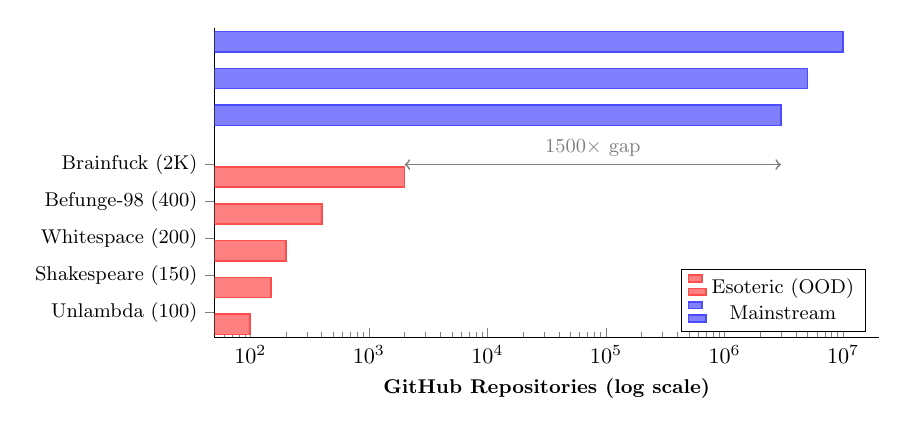
\begin{tikzpicture}[scale=0.8]
\begin{axis}[
    xbar,
    width=\columnwidth,
    height=6.5cm,
    xlabel={GitHub Repositories (log scale)},
    xlabel style={font=\small\bfseries},
    symbolic y coords={UL,Shk,WS,Bef,BF,Cpp,Java,Python},
    ytick=data,
    yticklabels={Unlambda (100), Shakespeare (150), Whitespace (200), Befunge-98 (400), Brainfuck (2K), C++ (3M), Java (5M), Python (10M)},
    y tick label style={font=\small},
    xmode=log,
    xmin=50, xmax=20000000,
    bar width=0.32cm,
    axis lines*=left,
    enlarge y limits=0.1,
    legend style={at={(0.98,0.02)}, anchor=south east, font=\small},
    point meta=explicit symbolic,
]
\addplot[fill=red!50, draw=red!70, line width=0.8pt] coordinates {(100,UL)[] (150,Shk)[] (200,WS)[] (400,Bef)[] (2000,BF)[]};
\addplot[fill=blue!50, draw=blue!70, line width=0.8pt] coordinates {(3000000,Cpp)[] (5000000,Java)[] (10000000,Python)[]};
\legend{Esoteric (OOD), Mainstream}
\draw[<->, thick, gray] (axis cs:2000,BF) -- (axis cs:3000000,BF) node[midway, above, font=\small] {1500$\times$ gap};
\end{axis}
\end{tikzpicture}
\end{center}
\caption{Training data scarcity (GitHub repositories, log scale). Esoteric languages have 1,000--100,000$\times$ less data than mainstream languages, making contamination economically irrational.}
\label{fig:datascarcity}
\end{figure}

\subsection{Why This Benchmark Matters}

The EsoLang benchmark embodies our core thesis: it is economically irrational to optimize for this benchmark. Training on esoteric language code would consume resources, degrade mainstream performance, and yield no deployment value. Unlike MMLU or HumanEval where benchmark gaming provides competitive advantage, success on EsoLang can only come from genuine reasoning transfer.

\section{Empirical Evidence: Current Models Fail on OOD Tasks}

We evaluated five frontier models---GPT-5.2, Gemini 3 Pro, O4-mini-high, Qwen3-235B, and Kimi K2---on our 80-problem dataset across all five esoteric languages. We tested three prompting strategies (zero-shot, few-shot with 3 examples, and self-scaffolding) plus two agentic systems with IDE integration (GPT-5.2 Codex and Claude Code Opus 4.5).

\subsection{Zero-Shot Results}

Table~\ref{tab:zeroshot} shows zero-shot performance where models receive only the problem description and language specification. The best model solves only 6 problems (1.5\% overall).

\begin{table}[t]
\caption{Zero-shot accuracy (\%) per language. All values represent percentage of 80 problems solved.}
\label{tab:zeroshot}
\vskip 0.05in
\begin{center}
\begin{small}
\begin{tabular}{lccccc}
\toprule
Model & BF & Bef & WS & UL & Shk \\
\midrule
GPT-5.2 & 2.5\% & 2.5\% & 0\% & 0\% & 2.5\% \\
Gemini 3 Pro & 2.5\% & 5.0\% & 0\% & 0\% & 0\% \\
O4-mini-high & 2.5\% & 0\% & 0\% & 0\% & 1.2\% \\
Kimi K2 & 0\% & 2.5\% & 0\% & 0\% & 1.2\% \\
Qwen3-235B & 2.5\% & 0\% & 0\% & 0\% & 0\% \\
\bottomrule
\end{tabular}
\end{small}
\end{center}
\end{table}

\subsection{Few-Shot Results}

Table~\ref{tab:fewshot} shows few-shot performance with 3 solved examples per language. Improvements are marginal (at most +1\% absolute), and some models show regression.

\begin{table}[t]
\caption{Few-shot accuracy (\%) with 3 examples. Minimal improvement over zero-shot.}
\label{tab:fewshot}
\vskip 0.05in
\begin{center}
\begin{small}
\begin{tabular}{lccccc}
\toprule
Model & BF & Bef & WS & UL & Shk \\
\midrule
GPT-5.2 & 2.5\% & 8.8\% & 0\% & 0\% & 1.2\% \\
Gemini 3 Pro & 3.8\% & 3.8\% & 0\% & 0\% & 0\% \\
O4-mini-high & 2.5\% & 0\% & 0\% & 0\% & 1.2\% \\
Kimi K2 & 0\% & 1.2\% & 0\% & 0\% & 1.2\% \\
Qwen3-235B & 1.2\% & 0\% & 0\% & 1.2\% & 0\% \\
\bottomrule
\end{tabular}
\end{small}
\end{center}
\end{table}

\subsection{Self-Scaffolding Results}

Self-scaffolding allows models to iteratively refine their solutions based on interpreter feedback. After each attempt, the model receives the interpreter's output (success, error message, or incorrect output) and can generate a new solution. We allow up to 5 attempts per problem. Crucially, no LLM-based critic or reflection prompt is used---models must learn purely from execution feedback.

Table~\ref{tab:selfscaffold} shows that even with iterative feedback, performance remains below 11\% per language. The best result (GPT-5.2 on Befunge at 10\%) still represents near-complete failure.

\begin{table}[t]
\caption{Self-scaffolding accuracy (\%) with 5 attempts and interpreter feedback.}
\label{tab:selfscaffold}
\vskip 0.05in
\begin{center}
\begin{small}
\begin{tabular}{lccccc}
\toprule
Model & BF & Bef & WS & UL & Shk \\
\midrule
GPT-5.2 & 6.2\% & 10.0\% & 0\% & 0\% & 2.5\% \\
Gemini 3 Pro & 5.0\% & 7.5\% & 0\% & 0\% & 1.2\% \\
Qwen3-235B & 2.5\% & 0\% & 0\% & 1.2\% & 1.2\% \\
O4-mini-high & 2.5\% & 0\% & 0\% & 0\% & 1.2\% \\
Kimi K2 & 0\% & 0\% & 0\% & 0\% & 1.2\% \\
\bottomrule
\end{tabular}
\end{small}
\end{center}
\end{table}

The results demonstrate that interpreter feedback alone cannot overcome fundamental knowledge gaps. Models cannot learn from error messages when they lack basic understanding of the target language's execution model.

\subsection{Agentic System Results}

We additionally evaluated two agentic systems with IDE integration and tool access on Brainfuck and Befunge-98 (Table~\ref{tab:agentic}). \textbf{GPT-5.2 Codex} operates via the OpenAI Codex API with direct interpreter access, while \textbf{Claude Code (Opus 4.5)} uses Claude Opus 4.5 with persistent context and interpreter feedback.

\begin{table}[t]
\caption{Agentic system accuracy (\%) on Brainfuck and Befunge-98. Both systems have IDE integration with direct interpreter access.}
\label{tab:agentic}
\vskip 0.05in
\begin{center}
\begin{small}
\begin{tabular}{lccc}
\toprule
System & BF & Bef & Avg \\
\midrule
Codex (IDE) & \textbf{13.8\%} & \textbf{8.8\%} & \textbf{11.2\%} \\
Claude Code (Opus 4.5) & 12.5\% & 8.8\% & 10.6\% \\
\bottomrule
\end{tabular}
\end{small}
\end{center}
\end{table}

Both IDE-integrated systems achieve 2--3$\times$ improvement over non-agentic approaches, with Codex reaching 13.8\% on Brainfuck---the highest single-language result. We attribute this to three architectural advantages: (1) \textbf{direct interpreter access} enabling tight feedback loops where execution results inform subsequent attempts without context degradation; (2) \textbf{efficient context management} with structured logging that mitigates the \textit{lost-in-the-middle} phenomenon~\cite{liu2024lost} by fetching relevant prior attempts rather than maintaining full conversation history; and (3) \textbf{task-specific ICL retrieval} providing relevant exemplars (e.g., solved string manipulation problems when attempting a new string task) rather than generic demonstrations.

\subsection{Why In-Context Learning Fails on OOD Tasks}

A critical finding across our experiments is that \textbf{few-shot learning provides negligible benefit} for truly out-of-distribution tasks. Comparing Tables~\ref{tab:zeroshot} and~\ref{tab:fewshot}, few-shot prompting shows no statistically significant improvement over zero-shot (average change $+0.8$ percentage points). This aligns with prior work showing that ICL effectiveness depends critically on pre-training data coverage~\cite{min2022rethinking}---demonstrations activate relevant pre-trained knowledge rather than teaching genuinely new skills.

When the target domain lies outside the pre-training corpus, demonstration examples cannot compensate for missing foundational knowledge. The minimal performance separation between zero-shot and few-shot conditions demonstrates that ICL examples serve primarily as retrieval cues for pre-trained patterns rather than enabling genuine task learning.

In contrast, agentic systems with interpreter-in-the-loop architecture substantially outperform standard prompting because they provide \textbf{empirical verification} rather than relying on pattern matching. The model receives concrete execution traces (actual vs.\ expected output, error messages, stack traces) rather than another model's interpretation of failures. For OOD tasks where the model lacks domain knowledge, direct interpreter feedback provides a sharper learning signal than textual demonstrations or self-reflection.

\subsection{Error Pattern Analysis}

Figure~\ref{fig:errors} shows the error distribution for GPT-5.2 zero-shot evaluation across all five languages. Brainfuck exhibits primarily \textbf{logic errors} (60\%)---models generate syntactically valid code but implement incorrect algorithms. Befunge-98 shows high \textbf{runtime errors} (45\%), indicating models attempt execution but misunderstand 2D grid program flow. In contrast, Whitespace and Unlambda are dominated by \textbf{compile errors} (90--100\%)---models cannot generate valid syntax even with documentation. Shakespeare shows 70\% compile errors as natural-language-like syntax misleads models into generating theatrical prose rather than valid programs.

\begin{figure}[t]
\begin{center}
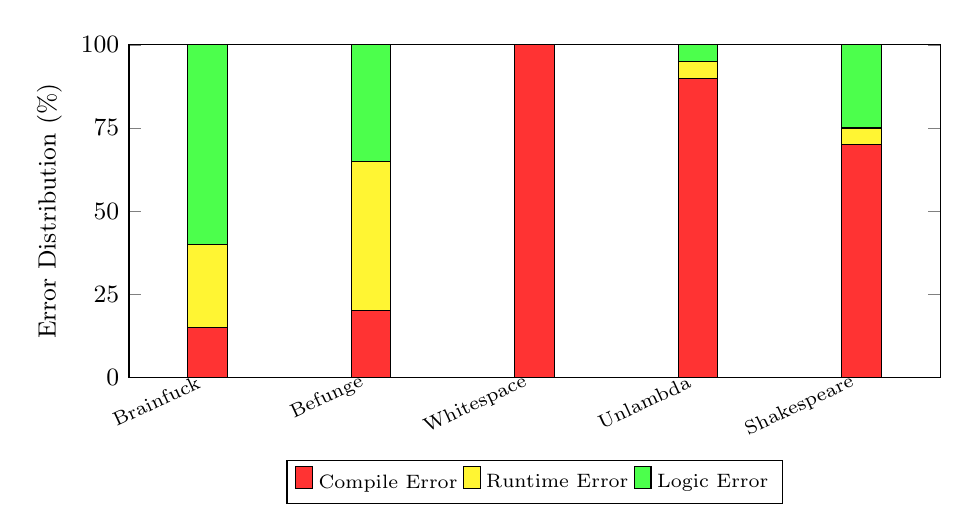
\begin{tikzpicture}
\begin{axis}[
    ybar stacked,
    bar width=0.5cm,
    width=0.98\columnwidth,
    height=5.8cm,
    ylabel={Error Distribution (\%)},
    ylabel style={font=\small},
    symbolic x coords={BF, Bef, WS, UL, Shk},
    xtick=data,
    xticklabels={Brainfuck, Befunge, Whitespace, Unlambda, Shakespeare},
    x tick label style={font=\scriptsize, rotate=25, anchor=east},
    ymin=0, ymax=100,
    ytick={0,25,50,75,100},
    y tick label style={font=\small},
    legend style={at={(0.5,-0.25)}, anchor=north, legend columns=3, font=\scriptsize},
    enlarge x limits=0.12,
]
\addplot[fill=red!80] coordinates {(BF,15) (Bef,20) (WS,100) (UL,90) (Shk,70)};
\addplot[fill=yellow!80] coordinates {(BF,25) (Bef,45) (WS,0) (UL,5) (Shk,5)};
\addplot[fill=green!70] coordinates {(BF,60) (Bef,35) (WS,0) (UL,5) (Shk,25)};
\legend{Compile Error, Runtime Error, Logic Error}
\end{axis}
\end{tikzpicture}
\end{center}
\caption{Error distribution by language (GPT-5.2 zero-shot). Languages with more training data (BF, Bef) show low compile errors but high logic/runtime errors. Extremely scarce languages (WS, UL) show 90--100\% compile errors.}
\label{fig:errors}
\end{figure}

\section{Test-Time Learning: From Taboo to Necessity}

Our benchmark proposal necessitates rethinking the role of learning during evaluation. We argue that test-time learning should be embraced as a core capability to measure, not forbidden as a violation of evaluation principles.

\subsection{The Paradigm is Emerging}

Recent work demonstrates the viability of test-time learning approaches. Test-Time Training (TTT) \cite{sun2020test} introduced the paradigm of adapting models at test time using self-supervised auxiliary tasks. Sun et al.~\cite{sun2024learning} extend this with RNNs that use expressive hidden states to learn at test time, while Yuksekgonul et al.~\cite{yuksekgonul2026discover} demonstrate learning to discover new knowledge during inference. TENT \cite{wang2021tent} proposed entropy minimization for lightweight test-time adaptation. More recently, Test-Time Reinforcement Learning (TTRL) \cite{zuo2025ttrl} achieved 211\% improvement on mathematical reasoning benchmarks by applying RL during inference using self-generated rewards.

These approaches demonstrate that significant capability improvements are possible without access to labeled training data, precisely the scenario our esoteric language benchmarks would evaluate. End-to-end test-time training formulates long-context modeling as continual learning, where models compress context into weights via next-token prediction during inference and use meta-learning at training time to prepare for test-time adaptation \cite{gandelsman2022test}.

\subsection{Architectural Requirements}

Test-time learning demands new architectural thinking that aligns with the decoupled paradigm we advocate. First, models require disentangled memory and reasoning components, meaning separate modules for static knowledge versus dynamic reasoning that can be updated without catastrophic forgetting \cite{kirkpatrick2017overcoming, wu2024continual}. Memory modules should support both short-term working memory and long-term consolidation, mirroring human cognitive architecture.

Second, efficient update mechanisms are essential. Parameter-efficient methods like LoRA \cite{hu2022lora} and adapters \cite{houlsby2019parameter} enable lightweight adaptation without full fine-tuning. QLoRA \cite{dettmers2023qlora} extends this with quantization for practical deployment. Sparse update patterns can preserve existing knowledge while acquiring new capabilities.

Third, meta-learning capabilities enable rapid adaptation \cite{finn2017model}. Training objectives should include test-time learning performance, not just immediate task accuracy. Models should learn to learn, optimizing not just for current performance but for adaptability to novel domains.

\subsection{Beyond Monolithic Models}

Our position challenges the prevailing assumption that a single ``monolithic'' foundation model should contain all knowledge. The continual learning literature has long established that single models cannot indefinitely accumulate knowledge without catastrophic forgetting, capacity saturation, or optimization collapse from conflicting gradients \cite{kirkpatrick2017overcoming, scialom2022fine}.

We advocate for specialized systems that learn dynamically. Rather than expecting models to have all knowledge baked in, we should develop task-specific models that excel in their domains while enabling test-time learning for novel tasks within those domains. This mirrors biological intelligence: humans are not monolithic. We have specialized brain regions, learn continuously throughout life, and appropriately forget rarely-used information.

\section{Proposed Evaluation Framework}

Based on our analysis, we propose a comprehensive evaluation framework for dynamic OOD benchmarks that shifts from measuring memorization to measuring learning capability.

\subsection{Benchmark Design Principles}

Effective dynamic benchmarks should measure multiple dimensions of learning capability. Learning efficiency captures time to achieve functional proficiency measured in tokens processed, problems attempted, and interpreter interactions required. Parameter update efficiency tracks which parameters change during test-time learning, the magnitude and sparsity of updates, and whether updates preserve performance on other tasks.

Accuracy-compute curves capture performance as a function of inference-time compute budget, enabling comparison with human learning curves and diminishing returns analysis. Feedback utilization measures ability to learn from interpreter errors, error correction across attempts, and meta-learning, specifically whether the model improves at learning new languages over time.

\subsection{Evaluation Protocol}

We propose a three-phase evaluation protocol. In Phase 1 (Documentation + Few-Shot), models receive language specifications and 3--5 solved example problems with no prior training on this material. In Phase 2 (Interactive Problem-Solving), models attempt problems with access to interpreters, receiving error messages and allowed to update approach or parameters across iterations until solution or timeout.

Phase 3 evaluates generalization across three dimensions: within-language generalization to new problems in the same language, meta-learning evaluation on problems in different esoteric languages, and catastrophic forgetting assessment by returning to mainstream language problems.

\begin{figure}[t]
\begin{center}
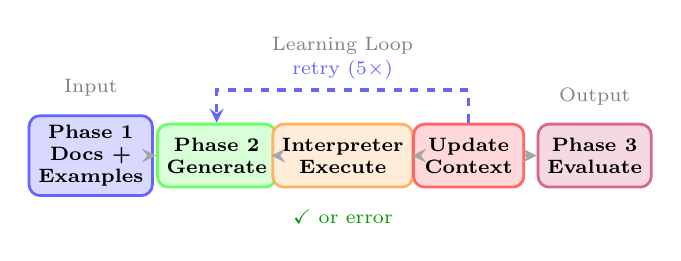
\begin{tikzpicture}[
    scale=0.64,
    phase/.style={rectangle, rounded corners=4pt, line width=1pt, minimum width=1.4cm, minimum height=0.8cm, font=\scriptsize\bfseries, align=center},
    arrow/.style={->, >=stealth, line width=1.2pt, gray!70}
]
% Phase 1
\node[phase, draw=blue!60, fill=blue!15] (p1) at (0,0) {Phase 1\\Docs +\\Examples};
% Phase 2
\node[phase, draw=green!60, fill=green!15] (p2) at (2.5,0) {Phase 2\\Generate};
\node[phase, draw=orange!60, fill=orange!15] (p3) at (5.0,0) {Interpreter\\Execute};
\node[phase, draw=red!60, fill=red!15] (p4) at (7.5,0) {Update\\Context};
% Phase 3
\node[phase, draw=purple!60, fill=purple!15] (p5) at (10.0,0) {Phase 3\\Evaluate};

% Arrows
\draw[arrow] (p1) -- (p2);
\draw[arrow] (p2) -- (p3);
\draw[arrow] (p3) -- (p4);
\draw[arrow] (p4) -- (p5);

% Retry loop
\draw[arrow, dashed, blue!60] (p4.north) -- ++(0,0.65) -| (p2.north) node[pos=0.25, above, font=\scriptsize] {retry (5$\times$)};

% Phase labels
\node[font=\scriptsize, gray, above=0.1cm of p1] {Input};
\node[font=\scriptsize, gray, above=0.75cm of p3] {Learning Loop};
\node[font=\scriptsize, gray, above=0.1cm of p5] {Output};

% Success/Fail annotation
\node[font=\scriptsize, green!60!black, below=0.15cm of p3] {$\checkmark$ or error};
\end{tikzpicture}
\end{center}
\caption{Test-time learning evaluation protocol: models receive documentation (Phase 1), then iteratively generate solutions with interpreter feedback (Phase 2), updating context until success or maximum attempts, followed by metric evaluation (Phase 3).}
\label{fig:protocol}
\end{figure}

\subsection{Metrics Beyond Accuracy}

Unlike traditional benchmarks reporting single accuracy numbers, our framework captures rich learning dynamics. We propose reporting solve rate versus attempts curves, inference-time compute consumed, parameter update magnitudes and locations, error type distributions across attempts, and generalization coefficients measuring transfer to new problems and languages.

\begin{figure}[t]
\begin{center}
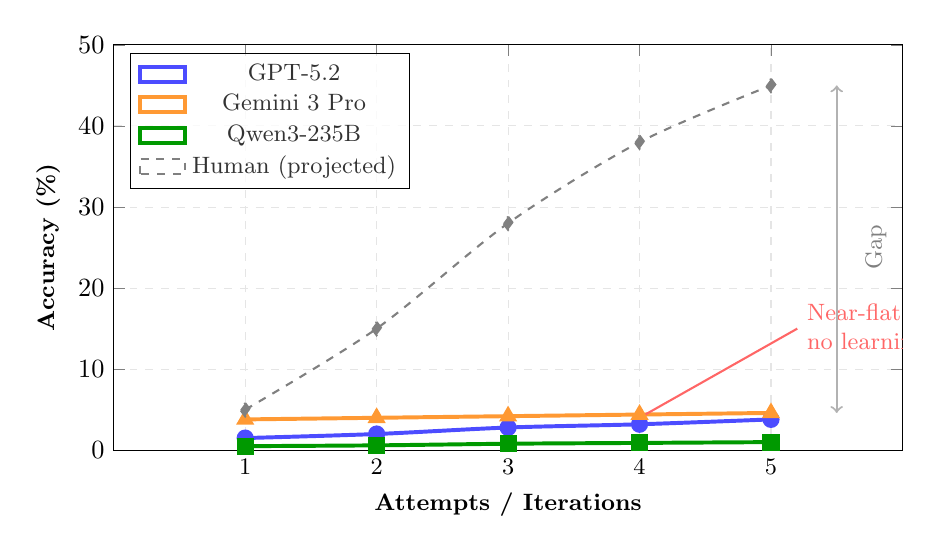
\begin{tikzpicture}[scale=0.95]
\begin{axis}[
    width=1.0\columnwidth,
    height=7cm,
    xlabel={Attempts / Iterations},
    ylabel={Accuracy (\%)},
    xlabel style={font=\small\bfseries},
    ylabel style={font=\small\bfseries},
    xmin=0, xmax=6, ymin=0, ymax=50,
    xtick={1,2,3,4,5},
    xticklabels={1,2,3,4,5},
    x tick label style={font=\small},
    ytick={0,10,20,30,40,50},
    legend style={at={(0.02,0.98)}, anchor=north west, font=\small, fill=white, fill opacity=0.8},
    grid=major, grid style={dashed, gray!20},
    area legend,
]
% GPT-5.2 - best performer
\addplot[thick, blue!70, smooth, mark=*, mark size=2.5pt, line width=1.5pt] coordinates {
    (1,1.5) (2,2.0) (3,2.8) (4,3.2) (5,3.8)
};
% Gemini 3 Pro
\addplot[thick, orange!80, smooth, mark=triangle*, mark size=2.5pt, line width=1.5pt] coordinates {
    (1,3.8) (2,4.0) (3,4.2) (4,4.4) (5,4.6)
};
% Qwen3-235B
\addplot[thick, green!60!black, smooth, mark=square*, mark size=2.5pt, line width=1.5pt] coordinates {
    (1,0.5) (2,0.6) (3,0.8) (4,0.9) (5,1.0)
};
% Theoretical human (for comparison)
\addplot[thick, gray, dashed, smooth, mark=diamond*, mark size=2.5pt] coordinates {
    (1,5) (2,15) (3,28) (4,38) (5,45)
};
\legend{GPT-5.2, Gemini 3 Pro, Qwen3-235B, Human (projected)}

% Annotation: flat learning curve
\draw[<-, thick, red!60] (axis cs:4,4) -- (axis cs:5.2,15) node[right, font=\small, align=left] {Near-flat:\\no learning};

% Gap annotation
\draw[<->, thick, gray!60] (axis cs:5.5,4.6) -- (axis cs:5.5,45);
\node[font=\small, gray, rotate=90] at (axis cs:5.8,25) {Gap};
\end{axis}
\end{tikzpicture}
\end{center}
\caption{Learning curves reveal minimal improvement across iterations. Current LLMs show near-flat trajectories (1--5\% accuracy regardless of attempts), while humans show steep learning. This gap represents the core capability deficit our benchmark exposes.}
\label{fig:learningcurve}
\end{figure}

\section{Alternative Views}
\label{sec:alternatives}

We acknowledge several credible positions opposed to our proposal and address each directly.

\textbf{``Esoteric languages are too niche to matter.''} This objection misunderstands our proposal's purpose. We do not advocate for building better Brainfuck programmers. Rather, esoteric languages serve as controlled probes for transferable reasoning precisely because their obscurity makes them ideal for evaluating generalization. The goal is measuring whether models can apply computational reasoning to novel domains, not whether they can produce useful esolang code.

\textbf{``Test-time training violates fundamental ML evaluation principles.''} This objection conflates evaluation paradigms. Traditional train-test separation remains appropriate for measuring memorized knowledge, but is inappropriate for measuring learning capability. Humans learn during ``test time'' constantly. The ability to learn from limited experience is a core aspect of intelligence we should measure, not forbid. Our proposal creates a new evaluation paradigm alongside, not replacing, traditional benchmarks.

\textbf{``The computational cost is prohibitive.''} While test-time learning evaluation requires more compute than single-pass inference, several factors mitigate this concern. Current benchmark gaming may waste more total compute through repeated training to optimize benchmark scores. Inference-time compute costs continue to decrease rapidly. We can create tiered benchmark suites with fast approximations for development and comprehensive evaluation for publication.

\textbf{``Models should not need to learn at test time; they should already know.''} This position assumes the goal is building omniscient systems with all knowledge pre-encoded. We argue this is neither achievable nor desirable. No finite model can contain all possible knowledge, and the real world constantly generates new domains, languages, and tasks. Systems that can learn and adapt are more aligned with practical deployment requirements and more similar to human intelligence.

\section{Call to Action}

We propose concrete steps for the machine learning community to realize our position's aims.

\textbf{For benchmark developers:} Develop and release a comprehensive esoteric language benchmark suite (EsoEval) with standardized evaluation protocols, interpreter integration, and test-time learning metrics. Establish private holdout sets maintained by trusted third parties that are never made public. Implement dynamic benchmark generation producing new problems algorithmically.

\textbf{For model developers:} Invest in architectures with disentangled memory and reasoning components. Develop efficient test-time adaptation mechanisms beyond current LoRA and prompt-tuning approaches. Report test-time learning metrics alongside static benchmark scores.

\textbf{For the research community:} Shift community norms to value capability evaluation over score optimization. Require test-time learning evaluation for claims of ``general'' intelligence. Develop theoretical frameworks for understanding what makes tasks learnable at test time versus requiring pre-training.

\section{Conclusion}

We present EsoLang, the first benchmark designed to evaluate \textit{transferable reasoning skills} rather than memorized knowledge---mimicking how humans acquire new abilities by learning online from feedback and applying general knowledge to unfamiliar domains. Our empirical results reveal that frontier models achieving 85--92\% on mainstream programming tasks score below 14\% on esoteric languages, with few-shot learning providing no benefit---confirming that in-context learning activates pre-trained knowledge rather than enabling genuine skill acquisition. Agentic systems with efficient context management and interpreter feedback achieve 2--3$\times$ improvement, suggesting feedback loops that mirror human trial-and-error learning offer a more promising path.

By making benchmark gaming economically irrational and measuring the ability to learn rather than retrieve, EsoLang provides an evaluation paradigm aligned with developing systems that genuinely adapt to novel domains.

\bibliography{references}
\bibliographystyle{icml2026}

\section*{Impact Statement}

This position paper advocates for fundamental changes in how the machine learning community evaluates language models. We discuss potential broader impacts of this work.

\textbf{Positive Impacts.} Our proposed evaluation paradigm could reduce benchmark gaming incentives that currently distort research priorities and inflate capability claims. By measuring genuine learning rather than memorization, evaluations would better predict real-world deployment performance, potentially improving AI system reliability. The focus on test-time learning aligns evaluation with developing AI systems that can safely adapt to novel situations---a key requirement for beneficial AI deployment.

\textbf{Potential Concerns.} Shifting to dynamic benchmarks requires more computational resources for evaluation, which could disadvantage researchers with limited compute access. We advocate for tiered benchmark suites with efficient approximations to mitigate this. Additionally, our emphasis on modular, continuously learning systems raises questions about oversight---systems that learn at deployment time may be harder to audit than static models. We believe this concern is better addressed through developing appropriate oversight mechanisms rather than avoiding the capability entirely.

\textbf{Dual-Use Considerations.} The esoteric programming languages we propose for evaluation have no practical applications that could enable misuse. The benchmark design principles we advocate---ungameable evaluation, test-time learning measurement, and modular architectures---are broadly applicable to improving AI safety evaluation rather than enabling harmful applications.

\newpage
\appendix
\onecolumn
\section{EsoLang Benchmark: Full Problem Categories}

Table~\ref{tab:full_problems} presents the complete categorization of the 80 problems in the EsoLang Benchmark Dataset.

\begin{table}[h]
\caption{Complete problem list for the EsoLang Benchmark Dataset organized by difficulty and category.}
\label{tab:full_problems}
\begin{center}
\begin{small}
\begin{tabular}{lll}
\toprule
ID & Title & Category \\
\midrule
\multicolumn{3}{l}{\textbf{Easy (E01--E20)}} \\
E01 & Print Hello World & Output \\
E02 & Echo Line & I/O \\
E03 & Hello Name & String Formatting \\
E04 & Sum Two Integers & Arithmetic \\
E05 & Multiply Two Integers & Arithmetic \\
E06 & Even Or Odd & Conditionals \\
E07 & String Length & String Processing \\
E08 & Reverse String & String Manipulation \\
E09 & Count Vowels & Character Counting \\
E10 & Sum From 1 To N & Loops \\
\midrule
\multicolumn{3}{l}{\textbf{Medium (M01--M20)}} \\
M01 & Palindrome Check & String Analysis \\
M03 & Run Length Encoding & String Compression \\
M04 & Caesar Shift By 3 & Character Mapping \\
M06 & Greatest Common Divisor & Number Theory \\
M07 & Factorial & Recursion/Loops \\
M08 & Nth Fibonacci Number & Dynamic Programming \\
M09 & Decimal To Binary & Base Conversion \\
M13 & Sort Numbers & Sorting \\
\midrule
\multicolumn{3}{l}{\textbf{Hard (H01--H20)}} \\
H01 & Balanced Parentheses & Stack Operations \\
H02 & Evaluate Expression & Parsing \\
H03 & Count Primes Up To N & Prime Sieving \\
H04 & Nth Prime Number & Prime Generation \\
H05 & Big Integer Addition & Arbitrary Precision \\
H09 & General Caesar Cipher & Modular Arithmetic \\
H13 & Polynomial Evaluation & Expression Evaluation \\
\midrule
\multicolumn{3}{l}{\textbf{Extra-Hard (X01--X20)}} \\
X01 & Prime Factorization & Factorization \\
X02 & Longest Increasing Subseq. & Dynamic Programming \\
X03 & Matrix Multiplication & Linear Algebra \\
X04 & Evaluate Postfix Expression & Stack-Based Eval \\
X07 & Longest Palindromic Substr. & String DP \\
X15 & Spiral Matrix Traversal & 2D Array Traversal \\
X17 & Roman To Integer & Parsing \\
X20 & Josephus Problem & Circular Lists \\
\bottomrule
\end{tabular}
\end{small}
\end{center}
\end{table}

\section{Evaluation Methodology Details}

\subsection{Model Configurations}

All experiments used the following model configurations:
\begin{itemize}
    \item \textbf{O3/O4-mini-high}: Default parameters with temperature 0.7 for generation
    \item \textbf{Gemini 3 Pro Preview}: Standard API configuration
    \item \textbf{GPT-5.2}: Temperature 0.7, top-p 0.95
\end{itemize}

For few-shot experiments, we provided 3 solved examples per language drawn from a held-out set of simple problems not included in the evaluation set.

\subsection{Interpreter Integration}

We integrated official or community-standard interpreters for each language:
\begin{itemize}
    \item \textbf{Brainfuck}: Standard memory-tape interpreter with 30,000-cell tape
    \item \textbf{Befunge-98}: Reference FBBI-compliant interpreter
    \item \textbf{Whitespace}: Standard Haskell reference implementation
    \item \textbf{Unlambda}: Reference C implementation
    \item \textbf{Shakespeare}: SPL compiler to C with execution
\end{itemize}

Each solution attempt was given a 10-second timeout. Solutions producing correct output for all 6 test cases were marked as passing.

\subsection{Prompting Strategy Details}

We employed three evaluation strategies:

\textbf{Zero-Shot:} Single generation attempt with problem description and language specification. No examples provided. 1 API call per problem.

\textbf{Few-Shot (3 Examples):} Problem description with 3 solved example problems in the target language. Examples selected from problems not in evaluation set. 1 API call per problem.

\textbf{Self-Scaffolding:} Iterative generation with interpreter feedback only. The model receives execution results (success/error messages) after each attempt and can refine its solution. Up to 5 attempts allowed, with 10-second timeout per execution. No LLM-based critique or self-reflection---only raw interpreter output.

\newpage
\section{Esoteric Language Specifications}
\label{sec:lang_details}

This appendix provides detailed specifications for each esoteric language in the EsoLang Benchmark.

\subsection{Brainfuck}

Brainfuck was created by Urban M\"uller in 1993, designed to have the smallest possible compiler. It operates on a memory tape of 30,000 cells initialized to zero, with a movable pointer. The entire language consists of only 8 commands:

\begin{itemize}
    \item \texttt{>} -- Move pointer right
    \item \texttt{<} -- Move pointer left
    \item \texttt{+} -- Increment current cell
    \item \texttt{-} -- Decrement current cell
    \item \texttt{[} -- Jump forward past matching \texttt{]} if cell is zero
    \item \texttt{]} -- Jump back to matching \texttt{[} if cell is nonzero
    \item \texttt{.} -- Output current cell as ASCII character
    \item \texttt{,} -- Input character and store in current cell
\end{itemize}

All other characters are ignored as comments. Despite its simplicity, Brainfuck is Turing-complete and can express any computation. Solving problems requires reasoning about pointer arithmetic, loop invariants, and memory layout without named variables, functions, or high-level control structures.

\subsection{Befunge-98}

Befunge-98 was created by Chris Pressey in 1993. Unlike conventional languages where code executes linearly, Befunge programs exist on a 2D grid where the instruction pointer can travel in four cardinal directions. Key commands include:

\begin{itemize}
    \item \texttt{>}, \texttt{v}, \texttt{<}, \texttt{\^{}} -- Set direction of travel (right, down, left, up)
    \item \texttt{\_} -- Horizontal branch: go right if top of stack is zero, else left
    \item \texttt{|}  -- Vertical branch: go down if top of stack is zero, else up
    \item \texttt{0}--\texttt{9} -- Push digit value onto stack
    \item \texttt{+}, \texttt{-}, \texttt{*}, \texttt{/}, \texttt{\%} -- Arithmetic operations
    \item \texttt{p} -- Put: pop y, x, v and store v at position (x,y) in the grid
    \item \texttt{g} -- Get: pop y, x and push the value at position (x,y)
    \item \texttt{.} -- Pop and output as integer
    \item \texttt{,} -- Pop and output as ASCII character
    \item \texttt{\&} -- Input integer
    \item \texttt{\~{}} -- Input character
    \item \texttt{@} -- End program
\end{itemize}

The \texttt{p} and \texttt{g} commands enable self-modifying code by reading and writing to the program grid. Success requires spatial reasoning and understanding non-linear program flow.

\subsection{Whitespace}

Whitespace was created by Edwin Brady and Kevin Hammond in 2003. Only three characters have meaning: space (S), tab (T), and newline (N). All other characters are ignored, meaning Whitespace programs can be hidden within other text. The language is stack-based with commands encoded as sequences:

\begin{itemize}
    \item \textbf{Stack Manipulation} (prefix S): push, duplicate, swap, discard
    \item \textbf{Arithmetic} (prefix TS): add, subtract, multiply, divide, modulo
    \item \textbf{Heap Access} (prefix TT): store, retrieve
    \item \textbf{Flow Control} (prefix N): labels, call, jump, conditional jumps, return, exit
    \item \textbf{I/O} (prefix TN): output character/number, read character/number
\end{itemize}

Numbers are encoded in binary using S (0) and T (1), terminated by N. This makes programs invisible to human readers and completely orthogonal to natural language patterns.

\subsection{Unlambda}

Unlambda was designed by David Madore in 1999 as a minimal functional programming language based on combinatory logic. It has no variables---only function application denoted by the backtick character. Core combinators:

\begin{itemize}
    \item \texttt{i} -- Identity: returns its argument unchanged
    \item \texttt{k} -- Constant: \texttt{`kx} returns a function that ignores its argument and returns x
    \item \texttt{s} -- Substitution: \texttt{```sxyz} computes \texttt{``xz`yz}
    \item \texttt{v} -- Void: absorbs any application, always returns v
    \item \texttt{.x} -- Print character x and return identity
    \item \texttt{r} -- Print newline
    \item \texttt{@} -- Read character from input
    \item \texttt{d} -- Delay evaluation (creates a ``promise'')
    \item \texttt{c} -- Call with current continuation
\end{itemize}

Even simple operations like integer arithmetic require constructing Church numerals through combinator compositions. Understanding Unlambda requires knowledge of lambda calculus and continuation-passing style.

\subsection{Shakespeare}

Shakespeare was created by Karl \r{A}slund and Jon Hasselstr\"om in 2001. Programs are written as theatrical plays with specific semantic mappings:

\begin{itemize}
    \item \textbf{Variables}: Characters declared in the dramatis personae (e.g., ``Romeo, a young man'')
    \item \textbf{Values}: Determined by adjectives---positive words (``beautiful'', ``fair'') contribute $+1$, negative words (``damned'', ``evil'') contribute $-1$, multiplied by 2 for each adjective. Nouns contribute base values.
    \item \textbf{Assignment}: ``You are as [adjective] as [expression]'' or ``You [noun]''
    \item \textbf{Control Flow}: Acts and scenes serve as labels; ``Let us proceed to scene III'' is a goto
    \item \textbf{Conditionals}: ``If so, let us proceed to act II'' (tests stack)
    \item \textbf{I/O}: ``Open your heart'' outputs a number; ``Speak your mind'' outputs ASCII; ``Listen to your heart'' inputs a number; ``Open your mind'' inputs ASCII
    \item \textbf{Stack}: ``Remember yourself'' pushes; ``Recall'' pops
\end{itemize}

Shakespeare tests whether models can parse computation from natural language that superficially resembles their training data but has entirely different semantics.

\end{document}
